\documentclass[11pt]{article}

% ============================================================
%  Packages
% ============================================================
\usepackage[utf8]{inputenc}
\usepackage[T1]{fontenc}
\usepackage{lmodern}

% Page geometry — arXiv-friendly single-column
\usepackage[margin=1in]{geometry}

% Math
\usepackage{amsmath,amssymb}

% Tables
\usepackage{booktabs}
\usepackage{multirow}
\usepackage{array}
\usepackage{tabularx}

% Figures
\usepackage{graphicx}
\usepackage{float}

% TikZ
\usepackage{tikz}
\usetikzlibrary{arrows.meta,positioning,calc,decorations.pathreplacing,shapes.geometric}

% Colors
\usepackage[dvipsnames]{xcolor}

% Bibliography (natbib for arXiv safety)
\usepackage[numbers,sort&compress]{natbib}

% Hyperlinks (after natbib)
\usepackage[colorlinks=true,linkcolor=MidnightBlue,citecolor=OliveGreen,urlcolor=BrickRed]{hyperref}

% Misc
\usepackage{enumitem}
\usepackage{microtype}
\usepackage{url}
\usepackage{xspace}

% ============================================================
%  Macros
% ============================================================
\newcommand{\ie}{\emph{i.e.}\@\xspace}
\newcommand{\eg}{\emph{e.g.}\@\xspace}
\newcommand{\cf}{\emph{cf.}\@\xspace}
\newcommand{\etal}{\emph{et~al.}\xspace}
\newcommand{\pullmode}{\textsc{Pull}\xspace}
\newcommand{\pushmode}{\textsc{Push}\xspace}

% ============================================================
%  Title
% ============================================================
\title{%
  Workflow Memory for Long-Horizon Agentic Composition:\\
  Architecture, Dual-Mode Retrieval, and Retrieval-Correction Signal%
}

\author{
  Vladimir Ovcharov\thanks{Correspondence: \texttt{volodymyr@legal.org.ua}.
    Repository: \url{https://github.com/overthelex/SecondLayer}.}\\
  LEX AI LLC, Kyiv, Ukraine\\
  \texttt{https://legal.org.ua}
}

\date{May 2026}

\begin{document}
\maketitle

% ============================================================
%  Abstract
% ============================================================
\begin{abstract}
Long-horizon agentic workflows---where a practitioner and an LLM co-author software over weeks to months---demand a memory substrate whose retrieval unit is the architectural decision, not the conversational turn or the code chunk, and whose refresh policy is dual-mode: pull-based for active sessions, push-based for dormant tasks.
Existing memory systems~\citep{packer2023memgpt, park2023generative, chhikara2025mem0} organize around dialogue episodes; code-RAG~\citep{zhang2023repocoder, wang2024coderagbench} retrieves over source text without decision provenance; long-context models~\citep{reid2024gemini} suffer attention degradation past ${\sim}200$K tokens~\citep{liu2023lost, hsieh2024ruler}.
None treats decision provenance as a first-class memory unit or provides a slow-loop refresh primitive.
We frame this memory layer as scalable oversight infrastructure: retrieval-correction edits---practitioner corrections that would have been unnecessary had memory surfaced relevant context---constitute a process-level oversight signal that scales with agent autonomy, complementing outcome-level preference data.

This paper makes three contributions.
First, a \emph{three-layer memory decomposition}---domain, workflow, and practitioner---with distinct retrieval semantics per layer.
Second, \emph{dual-mode retrieval} as a first-class architectural primitive: pull mode fires at session start and queries all layers in parallel; push mode refreshes memory entries for dormant tasks proportional to repository activity, so that pull queries return current context even after weeks of inactivity.
Third, \emph{retrieval-correction edits} as a process-level oversight signal: corrections that operationalize the gap between the agent's available context and the context required for correct action, denser than outcome-level supervision and scaling with agent autonomy~\citep{ovcharov2026recursive}.
The architecture is deployed on a legal-technology platform (70+ MCP tools, 380M+ records, 1{,}547 merged PRs in 105 days).
Baseline measurements from 304 sessions confirm a median bootstrap cost of 30{,}115 input tokens and a median context waste ratio of 60\%; the memory layer targets a reduction to ${\leq}10$K tokens with ${\leq}20\%$ waste.
\end{abstract}

% ============================================================
\section{Introduction}
\label{sec:intro}
% ============================================================

A single practitioner, working recursively with Claude Code as the primary agentic engineering counterpart, shipped 1{,}547 merged pull requests across seven interconnected projects in 105 days~\citep[\S1]{ovcharov2026recursive}.
The system under construction---a legal-technology platform with 70+ MCP tools, 380M+ indexed records, and production customers---is not a toy benchmark.
It is an operational regime where architectural decisions made in week two constrain implementation choices in week six, where validator definitions evolve alongside the code they protect, and where the practitioner's correction history encodes domain expertise that no context window can hold indefinitely.

This operational regime is not served by existing memory or retrieval approaches.

\paragraph{CLAUDE.md scales as hand-curation.}
The dominant workaround for cross-session context in agentic workflows is a flat Markdown file (\texttt{CLAUDE.md}) that accumulates project conventions, architectural notes, and operational constraints.
In practice, its size grows linearly with project age: over 85 days and 25 commits, the \texttt{CLAUDE.md} for the platform described above grew from 4{,}099 to 24{,}148 characters at a rate of 217 characters/day ($R^2 = 0.87$ on a linear fit; see Section~\ref{sec:preliminary}).
A new session loads the entire file regardless of task relevance, wasting context budget on content that is irrelevant to the current task and out of date with respect to recent changes.
Worse, the practitioner bears the curation burden: every architectural decision must be manually distilled into the file, and stale entries silently degrade session quality.

\paragraph{Long context is not the answer.}
Models with 1M-token context windows~\citep{reid2024gemini} appear to eliminate the need for retrieval.
Empirically, they do not.
Attention degradation past ${\sim}200$K tokens is well documented: the ``lost in the middle'' effect causes models to underweight information in the interior of long contexts~\citep{liu2023lost}, and synthetic benchmarks like RULER confirm that effective context utilization degrades with length~\citep{hsieh2024ruler}.
Even where the context fits, cost scales with total context length, not with the relevance of individual entries.
At the 6-week horizon, the accumulated working set---prior decisions, rejected alternatives, validator evolution, constitutional principle invocations---exceeds what fits efficiently in any context window.

\paragraph{Conversational-agent memory is the wrong shape.}
MemGPT~\citep{packer2023memgpt}, Generative Agents~\citep{park2023generative}, A-MEM~\citep{xu2024amem}, and Mem0~\citep{chhikara2025mem0} organize memory around dialogue episodes: episodic recall of prior conversations, semantic memory for persistent facts, and reflection for self-assessment.
The retrieval unit is the conversational turn or the character observation.
None of these systems is designed for decision provenance---the record of which architectural alternative was chosen over which other, which constitutional principle was invoked, and which validator caught which class of regression.

\paragraph{Outcome-level supervision becomes thin at scale.}
As coding agents take on longer-horizon work---Anthropic Engineering documents agent sessions spanning thousands of context windows on a single project~\citep{anthropic2026harnesses}---outcome-level signal (did the shipped code work?) becomes a sparse, lagging indicator.
A single binary outcome may correspond to hours of agent activity and dozens of architectural micro-decisions.
Anthropic's published research priorities identify scalable oversight as a central open problem: how to design oversight mechanisms whose signal density grows with agent capability rather than degrading~\citep{anthropic2025recommended}.
This paper contributes a substrate for one such mechanism.
The memory layer's retrieval-correction edits are process-level oversight signals: each one identifies a specific gap between the context the agent had and the context the practitioner had, localized to a single edit.
Unlike outcome-level signals, retrieval-correction signals are produced continuously throughout a session, and their generation rate is invariant to session duration.

\medskip

This paper provides the mechanism for two conditions stated but not mechanized in the companion paper~\citep[\S2]{ovcharov2026recursive}: (1)~the codebase as persistent context, and (2)~compositional task layering across multi-week horizons.
The contributions are:

\begin{enumerate}[leftmargin=*, nosep]
  \item A \textbf{three-layer memory decomposition}---domain, workflow, and practitioner---with distinct retrieval semantics per layer (Section~\ref{sec:architecture}).
  \item \textbf{Dual-mode pull/push retrieval} as a first-class architectural primitive, where push-mode refresh keeps dormant-task memory current without requiring active sessions (Section~\ref{sec:dual-mode}).
  \item \textbf{Retrieval-correction edits} as a process-level oversight signal that scales with agent autonomy (Section~\ref{sec:retrieval-correction}). Each retrieval-correction edit localizes a specific context gap; aggregated across sessions, these edits constitute a dense oversight signal that complements the sparse outcome-level signal used in standard RLHF, and connects to the alignment pipeline described in the companion paper~\citep{ovcharov2026recursive}.
\end{enumerate}

The evaluation plan (Section~\ref{sec:evaluation}) defines measurable targets against instrumented baselines from the companion paper's dataset.
The architecture is designed for a single-practitioner regime and does not claim generality to multi-developer teams; limitations are discussed in Section~\ref{sec:limitations}.


% ============================================================
\section{Related Work}
\label{sec:related}
% ============================================================

% --------------------------------------------------
\subsection{Memory for Conversational Agents}
\label{sec:related-memory}
% --------------------------------------------------

The recent proliferation of LLM agents has produced a family of memory architectures organized around dialogue persistence.
MemGPT~\citep{packer2023memgpt} virtualizes a memory hierarchy analogous to an operating system's paging mechanism: a fixed main-context window is backed by an unbounded ``archival storage'' that the agent can read from and write to via self-directed function calls.
Generative Agents~\citep{park2023generative} introduced a three-part memory stream---observation, reflection, and planning---enabling simulated characters to maintain coherent behavior over extended interactions.
A-MEM~\citep{xu2024amem} extends this with Zettelkasten-inspired atomic notes and explicit inter-note linking.
Mem0~\citep{chhikara2025mem0} targets production deployment with a graph-based memory layer that supports multi-user, multi-session persistence.
A comprehensive survey of memory mechanisms for LLM agents appears in~\citet{zhang2024survey}.

Letta~\citep{letta2025lettacode}, the productized successor to MemGPT, advances the architecture in two directions relevant to this paper.
First, \emph{context repositories}~\citep{letta2026repositories}: persistent, versioned stores of structured context that agents read from and write to across sessions, replacing the flat archival-storage model with typed, queryable collections.
Second, \emph{context constitution}~\citep{letta2026constitution}: a declarative specification of what context an agent should have access to and how it should be prioritized, analogous to a retrieval policy expressed as a configuration rather than code.
These mechanisms move agent memory closer to the decision-provenance retrieval described here---context repositories provide the storage substrate, and context constitution provides a rudimentary retrieval policy.
However, Letta's retrieval unit remains the context block (a text chunk with metadata), not the architectural decision with provenance, alternatives, and constitutional anchoring.
The context constitution specifies \emph{which} collections to query, not \emph{what decision context} to retrieve for a given task.

These systems share a common retrieval unit: the conversational turn, the character observation, or the context block---closer to the architectural decision than turns or observations, but still without the explicit alternatives, validators, and constitutional anchoring that decision provenance requires.
They excel at role consistency, preference tracking, and episodic recall.
They are not designed for the retrieval unit that matters in long-horizon agentic engineering: the architectural decision with full provenance---which alternative was chosen, which was rejected, why, which validator enforces the choice, and which constitutional principle anchors it.

% --------------------------------------------------
\subsection{Retrieval-Augmented Code Agents}
\label{sec:related-code-rag}
% --------------------------------------------------

Code-RAG systems retrieve over source text to augment code generation.
RepoCoder~\citep{zhang2023repocoder} iteratively retrieves similar code snippets from the repository to improve completion accuracy.
CodeRAG-Bench~\citep{wang2024coderagbench} provides a systematic benchmark for retrieval-augmented code generation across documentation, API references, and code examples.
Commercial systems like Cursor's codebase indexing and Sourcegraph Cody build semantic indices over entire repositories, enabling natural-language queries that return relevant code chunks.
SWE-bench~\citep{jimenez2024swebench} and SWE-agent~\citep{yang2024sweagent} evaluate agents on real-world GitHub issues, demonstrating that retrieval over repository structure and issue context improves resolution rates.

All of these systems retrieve over \emph{code text and identifiers}.
They can answer ``where is this function defined?'' or ``what does this module do?'' but not ``why was this approach chosen over the alternative?'' or ``which constitutional principle does this validator enforce?''
The decision context---the rationale, the rejected alternatives, the cross-cutting constraints---is absent from the code itself and therefore absent from code-RAG retrieval.

% --------------------------------------------------
\subsection{Architecture Decision Records}
\label{sec:related-adr}
% --------------------------------------------------

The practice of recording architectural decisions has a long history in software engineering.
Nygard's Architecture Decision Record (ADR) format~\citep{nygard2011adr} proposes a lightweight Markdown template---title, status, context, decision, consequences---stored alongside the codebase.
The ISO/IEC/IEEE~42010 standard~\citep{iso42010} formalizes architecture description at the organizational level.
Z\"orner's Y-statement format~\citep{zorner2015softwarearchitekturen} structures decisions as ``In the context of [situation], facing [concern], we decided [option], to achieve [quality], accepting [downside].''
\citet{zimmermann2015architectural} extends ADR management to cross-project guidance with problem-space modeling.

ADRs capture decision provenance---exactly the content missing from code-RAG.
However, ADR retrieval is file-path-based: decisions are found by browsing a directory, not by semantic query.
There is no embedding index, no hybrid retrieval, no re-ranking by relevance to a current task.
ADRs also require manual authoring; in a high-velocity workflow producing 14.7~PRs/day, the curation overhead of maintaining a complete ADR directory is prohibitive.

% --------------------------------------------------
\subsection{Long-Context Language Models as a Substitute}
\label{sec:related-longcontext}
% --------------------------------------------------

Gemini~1.5~\citep{reid2024gemini} demonstrated effective processing of inputs up to 10M tokens in controlled settings.
This has led to a common assumption that sufficiently large context windows eliminate the need for retrieval.

Empirical evidence does not support this assumption for the regime considered here.
\citet{liu2023lost} showed that model performance degrades significantly for information placed in the middle of long contexts---the ``lost in the middle'' effect---even for models explicitly designed for long inputs.
RULER~\citep{hsieh2024ruler} confirmed that effective context utilization drops sharply as input length grows, with most models failing to maintain claimed context lengths under adversarial probing.
\citet{li2024longcontextbench} demonstrated that in-context learning performance degrades as the number of demonstrations grows, even when the total context fits within the window.

Beyond attention degradation, long-context processing is expensive.
At the 6-week horizon of the operational regime described here, the accumulated decision context---ADRs, validator histories, constitutional principle invocations, edit-trace summaries---would consume hundreds of thousands of tokens per session start.
Retrieval selects the task-relevant subset; long context pays for everything.

\medskip

\noindent\textbf{Synthesis.}
None of the four lines of work treats decision provenance as a first-class memory unit with semantic retrieval.
None provides a slow-loop refresh primitive that keeps dormant-task memory current across multi-week horizons.
The architecture described in this paper occupies the intersection: it adopts the provenance structure of ADRs, the semantic retrieval of code-RAG, the persistence of conversational memory systems, and the selective context loading of RAG---while adding dual-mode retrieval as a new architectural primitive.


% ============================================================
\section{Problem Formalization}
\label{sec:problem}
% ============================================================

Long-horizon agentic composition is a regime characterized by three measurable properties, verified in the companion paper's pilot dataset~\citep[\S3--4]{ovcharov2026recursive}:

\begin{description}[leftmargin=1.5em, nosep]
  \item[Horizon.] Related decisions span weeks to months. The platform described here maintained active development across 105 days with a median inter-PR interval under 2~hours but architectural threads that persisted for 4--6 weeks.
  \item[Compositionality.] Decision~$A$ in week~2 constrains decision~$B$ in week~6. A choice of database schema in the EDRSR import pipeline determined the parameter contract of 29 MCP tools built over the following five weeks; a constitutional principle established in week~1 governed validator behavior through week~15.
  \item[Persistence.] The codebase and its associated decision graph serve as shared state between sessions, not transient context. The agent does not carry forward a dialogue history; it re-enters a changed codebase each session.
\end{description}

\paragraph{The session bootstrap problem.}
Each new agentic session begins by loading context.
The agent consumes $T$ input tokens of \texttt{CLAUDE.md} content and system context automatically, then performs $K$ exploratory file reads before beginning productive work.
Measured across 304 sessions from the companion paper's dataset (Section~\ref{sec:preliminary}): median bootstrap cost is $T = 30{,}115$ input tokens, of which ${\sim}17{,}600$ (59\%) is cache-creation cost for \texttt{CLAUDE.md} alone; median per-session file reads are $K = 14$ (mean 23.1).
Both quantities grow with project age as \texttt{CLAUDE.md} accumulates conventions and the agent's file-read heuristics expand.

The relevant subset for any given task is a small fraction of $K$ and $T$.
Measured across 180 sessions with at least three bootstrap reads: the median \emph{context waste ratio}---files read but never subsequently edited---is 60\%, with source-code reads wasted at 78\% (Section~\ref{sec:preliminary}).
A task touching the billing service does not need the EDRSR import pipeline's conventions; a task modifying the frontend router does not need the PostgreSQL migration patterns.
Yet the flat bootstrap loads everything, because the agent cannot predict which subset is relevant without first loading the full context.

\paragraph{Pull-based retrieval reduces $K$ and $T$.}
A memory query replaces the flat bootstrap: the task description is embedded, matched against a pre-indexed memory store, and the top-$k$ relevant entries are assembled into a compact digest.
The agent starts with a focused context ($K' \ll K$, $T' \ll T$) and can retrieve additional entries on demand via MCP tool calls.

\paragraph{Push-based refresh keeps the substrate current.}
Pull-based retrieval alone fails for tasks that are dormant for weeks and then resume.
During the dormant period, other tasks' decisions accumulate context that is relevant to the dormant task---schema changes, principle additions, validator updates---but no pull query fires to incorporate this context.
When the dormant task resumes, the pull query retrieves stale entries from the last active period.
Push-mode refresh addresses this: a scheduled process watches task activity and refreshes memory entries for dormant tasks proportional to the rate of relevant changes, so that pull queries on resumption return current context.


% ============================================================
\section{Architecture}
\label{sec:architecture}
% ============================================================

The workflow memory service decomposes into three layers, each with distinct content, retrieval semantics, and storage substrate.
Figure~\ref{fig:architecture} shows the overall architecture with both retrieval modes.

% Three-layer workflow memory architecture with dual-mode retrieval
% Compile standalone: pdflatex architecture.tex
% Or include via % Three-layer workflow memory architecture with dual-mode retrieval
% Compile standalone: pdflatex architecture.tex
% Or include via % Three-layer workflow memory architecture with dual-mode retrieval
% Compile standalone: pdflatex architecture.tex
% Or include via \input{figures/architecture} from main.tex
\begin{figure}[t]
\centering
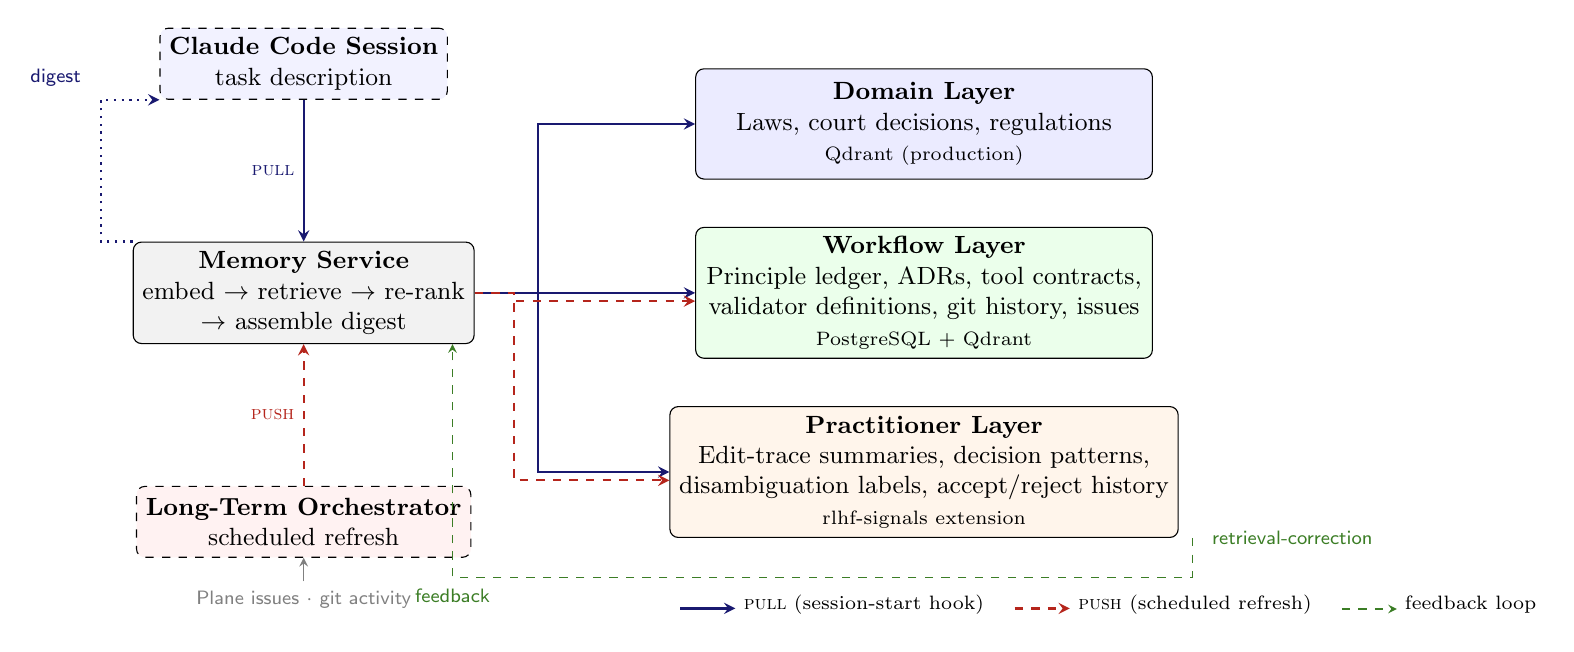
\begin{tikzpicture}[
    >=stealth,
    node distance=1.2cm and 2.0cm,
    layer/.style={draw, rounded corners=3pt, minimum width=5.8cm,
                  minimum height=1.4cm, align=center, font=\small},
    service/.style={draw, rounded corners=3pt, minimum width=3.8cm,
                    minimum height=1.0cm, align=center, font=\small},
    agent/.style={draw, dashed, rounded corners=3pt, minimum width=3.0cm,
                  minimum height=0.9cm, align=center, font=\small},
    pullpath/.style={->, thick, color=MidnightBlue},
    pushpath/.style={->, thick, color=BrickRed, dashed},
    labelbox/.style={font=\scriptsize\sffamily, fill=white, inner sep=1pt},
  ]

  % === Layers (right side) ===
  \node[layer, fill=blue!8] (domain)
    {\textbf{Domain Layer}\\Laws, court decisions, regulations\\{\scriptsize Qdrant (production)}};

  \node[layer, fill=green!8, below=0.6cm of domain] (workflow)
    {\textbf{Workflow Layer}\\Principle ledger, ADRs, tool contracts,\\
     validator definitions, git history, issues\\
     {\scriptsize PostgreSQL + Qdrant}};

  \node[layer, fill=orange!8, below=0.6cm of workflow] (practitioner)
    {\textbf{Practitioner Layer}\\Edit-trace summaries, decision patterns,\\
     disambiguation labels, accept/reject history\\
     {\scriptsize rlhf-signals extension}};

  % === Memory Service (center-left) ===
  \node[service, fill=gray!10, left=2.8cm of workflow] (memservice)
    {\textbf{Memory Service}\\embed $\rightarrow$ retrieve $\rightarrow$ re-rank\\$\rightarrow$ assemble digest};

  % === Claude Code session (top-left) ===
  \node[agent, fill=blue!5, above=1.8cm of memservice] (session)
    {\textbf{Claude Code Session}\\task description};

  % === Long-term orchestrator (bottom-left) ===
  \node[agent, fill=red!5, below=1.8cm of memservice] (orchestrator)
    {\textbf{Long-Term Orchestrator}\\scheduled refresh};

  % === Pull path (blue, solid) ===
  \draw[pullpath] (session.south) -- node[labelbox, left, xshift=-2pt]
    {\color{MidnightBlue}\textsc{pull}} (memservice.north);

  \draw[pullpath] (memservice.east) -- ++(0.8,0) |- (domain.west);
  \draw[pullpath] (memservice.east) -- (workflow.west);
  \draw[pullpath] (memservice.east) -- ++(0.8,0) |- (practitioner.west);

  % Return digest (pull)
  \draw[pullpath, dotted] (memservice.north west) -- ++(-0.4,0)
    |- node[labelbox, left, xshift=-6pt, yshift=8pt]
    {\color{MidnightBlue}digest} (session.south west);

  % === Push path (red, dashed) ===
  \draw[pushpath] (orchestrator.north) -- node[labelbox, left, xshift=-2pt]
    {\color{BrickRed}\textsc{push}} (memservice.south);

  \draw[pushpath] (memservice.east) -- ++(0.5,0) |- ([yshift=-3pt]workflow.west);
  \draw[pushpath] (memservice.east) -- ++(0.5,0) |- ([yshift=-3pt]practitioner.west);

  % === Issue tracker feed into orchestrator ===
  \node[font=\scriptsize\sffamily, below=0.3cm of orchestrator, text=gray]
    (tracker) {Plane issues $\cdot$ git activity};
  \draw[->, thin, gray] (tracker.north) -- (orchestrator.south);

  % === Retrieval-correction feedback loop ===
  \node[font=\scriptsize\sffamily, right=0.3cm of practitioner.south east,
        text=OliveGreen, anchor=west] (rcloop) {retrieval-correction};
  \draw[->, thin, OliveGreen, dashed]
    ([xshift=5pt]practitioner.south east) -- ++(0,-0.5)
    -| node[labelbox, below, yshift=-3pt] {\color{OliveGreen}feedback}
    ([xshift=-8pt]memservice.south east);

  % === Legend ===
  \node[anchor=north west, font=\scriptsize] at ([yshift=-0.6cm]practitioner.south west)
  {
    \tikz\draw[pullpath] (0,0) -- (0.7,0); \textsc{pull} (session-start hook) \quad
    \tikz\draw[pushpath] (0,0) -- (0.7,0); \textsc{push} (scheduled refresh) \quad
    \tikz\draw[->, thin, OliveGreen, dashed] (0,0) -- (0.7,0); feedback loop
  };

\end{tikzpicture}
\caption{Three-layer workflow memory architecture with dual-mode retrieval.
  \textsc{Pull} mode (solid blue) fires at session start: the task description is embedded
  and used to query all three Qdrant collections in parallel; results are re-ranked and
  assembled into a compact digest.
  \textsc{Push} mode (dashed red) runs on a schedule proportional to task activity,
  refreshing workflow and practitioner layer entries so that pull queries return current context.
  The retrieval-correction feedback loop (green) detects memory entries that \emph{should}
  have been retrieved but were not, feeding back into retrieval tuning and the RLHF
  pipeline as a process-level oversight signal.}
\label{fig:architecture}
\end{figure}
 from main.tex
\begin{figure}[t]
\centering
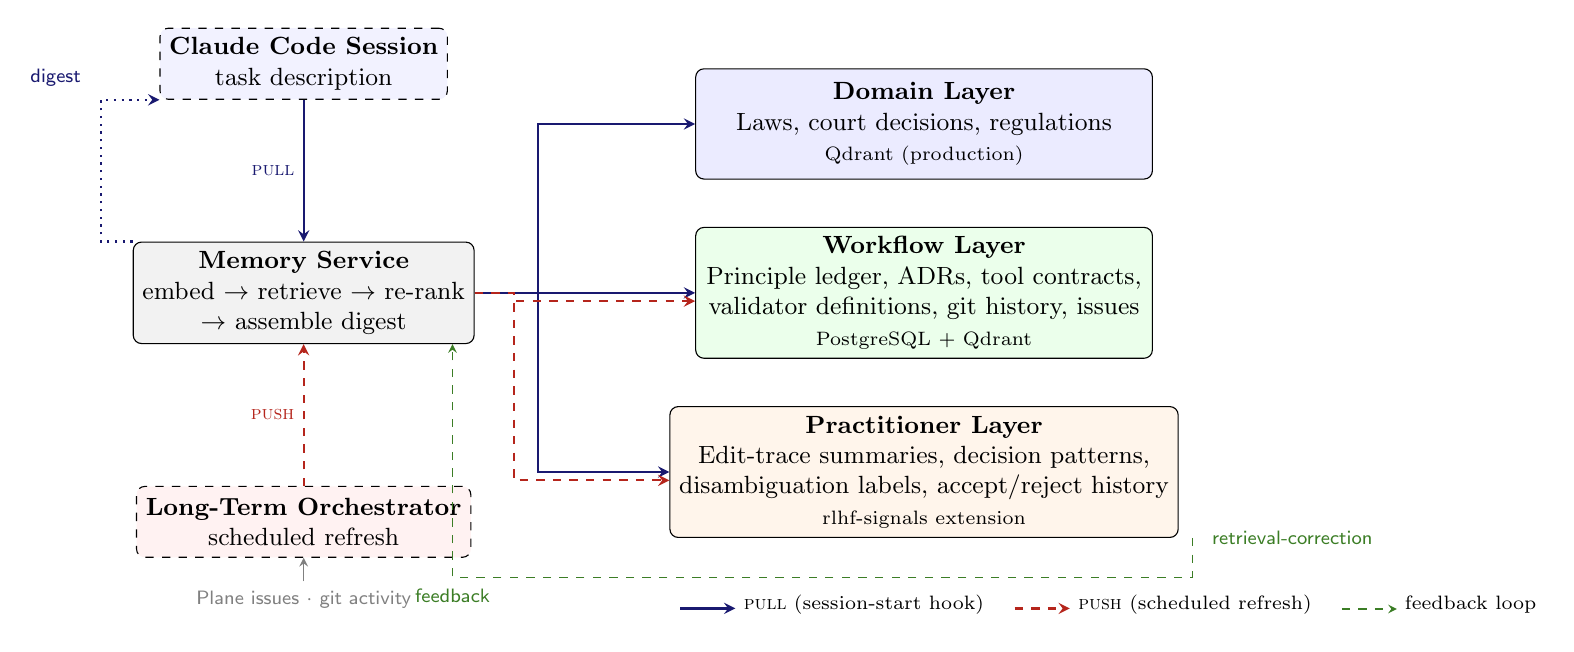
\begin{tikzpicture}[
    >=stealth,
    node distance=1.2cm and 2.0cm,
    layer/.style={draw, rounded corners=3pt, minimum width=5.8cm,
                  minimum height=1.4cm, align=center, font=\small},
    service/.style={draw, rounded corners=3pt, minimum width=3.8cm,
                    minimum height=1.0cm, align=center, font=\small},
    agent/.style={draw, dashed, rounded corners=3pt, minimum width=3.0cm,
                  minimum height=0.9cm, align=center, font=\small},
    pullpath/.style={->, thick, color=MidnightBlue},
    pushpath/.style={->, thick, color=BrickRed, dashed},
    labelbox/.style={font=\scriptsize\sffamily, fill=white, inner sep=1pt},
  ]

  % === Layers (right side) ===
  \node[layer, fill=blue!8] (domain)
    {\textbf{Domain Layer}\\Laws, court decisions, regulations\\{\scriptsize Qdrant (production)}};

  \node[layer, fill=green!8, below=0.6cm of domain] (workflow)
    {\textbf{Workflow Layer}\\Principle ledger, ADRs, tool contracts,\\
     validator definitions, git history, issues\\
     {\scriptsize PostgreSQL + Qdrant}};

  \node[layer, fill=orange!8, below=0.6cm of workflow] (practitioner)
    {\textbf{Practitioner Layer}\\Edit-trace summaries, decision patterns,\\
     disambiguation labels, accept/reject history\\
     {\scriptsize rlhf-signals extension}};

  % === Memory Service (center-left) ===
  \node[service, fill=gray!10, left=2.8cm of workflow] (memservice)
    {\textbf{Memory Service}\\embed $\rightarrow$ retrieve $\rightarrow$ re-rank\\$\rightarrow$ assemble digest};

  % === Claude Code session (top-left) ===
  \node[agent, fill=blue!5, above=1.8cm of memservice] (session)
    {\textbf{Claude Code Session}\\task description};

  % === Long-term orchestrator (bottom-left) ===
  \node[agent, fill=red!5, below=1.8cm of memservice] (orchestrator)
    {\textbf{Long-Term Orchestrator}\\scheduled refresh};

  % === Pull path (blue, solid) ===
  \draw[pullpath] (session.south) -- node[labelbox, left, xshift=-2pt]
    {\color{MidnightBlue}\textsc{pull}} (memservice.north);

  \draw[pullpath] (memservice.east) -- ++(0.8,0) |- (domain.west);
  \draw[pullpath] (memservice.east) -- (workflow.west);
  \draw[pullpath] (memservice.east) -- ++(0.8,0) |- (practitioner.west);

  % Return digest (pull)
  \draw[pullpath, dotted] (memservice.north west) -- ++(-0.4,0)
    |- node[labelbox, left, xshift=-6pt, yshift=8pt]
    {\color{MidnightBlue}digest} (session.south west);

  % === Push path (red, dashed) ===
  \draw[pushpath] (orchestrator.north) -- node[labelbox, left, xshift=-2pt]
    {\color{BrickRed}\textsc{push}} (memservice.south);

  \draw[pushpath] (memservice.east) -- ++(0.5,0) |- ([yshift=-3pt]workflow.west);
  \draw[pushpath] (memservice.east) -- ++(0.5,0) |- ([yshift=-3pt]practitioner.west);

  % === Issue tracker feed into orchestrator ===
  \node[font=\scriptsize\sffamily, below=0.3cm of orchestrator, text=gray]
    (tracker) {Plane issues $\cdot$ git activity};
  \draw[->, thin, gray] (tracker.north) -- (orchestrator.south);

  % === Retrieval-correction feedback loop ===
  \node[font=\scriptsize\sffamily, right=0.3cm of practitioner.south east,
        text=OliveGreen, anchor=west] (rcloop) {retrieval-correction};
  \draw[->, thin, OliveGreen, dashed]
    ([xshift=5pt]practitioner.south east) -- ++(0,-0.5)
    -| node[labelbox, below, yshift=-3pt] {\color{OliveGreen}feedback}
    ([xshift=-8pt]memservice.south east);

  % === Legend ===
  \node[anchor=north west, font=\scriptsize] at ([yshift=-0.6cm]practitioner.south west)
  {
    \tikz\draw[pullpath] (0,0) -- (0.7,0); \textsc{pull} (session-start hook) \quad
    \tikz\draw[pushpath] (0,0) -- (0.7,0); \textsc{push} (scheduled refresh) \quad
    \tikz\draw[->, thin, OliveGreen, dashed] (0,0) -- (0.7,0); feedback loop
  };

\end{tikzpicture}
\caption{Three-layer workflow memory architecture with dual-mode retrieval.
  \textsc{Pull} mode (solid blue) fires at session start: the task description is embedded
  and used to query all three Qdrant collections in parallel; results are re-ranked and
  assembled into a compact digest.
  \textsc{Push} mode (dashed red) runs on a schedule proportional to task activity,
  refreshing workflow and practitioner layer entries so that pull queries return current context.
  The retrieval-correction feedback loop (green) detects memory entries that \emph{should}
  have been retrieved but were not, feeding back into retrieval tuning and the RLHF
  pipeline as a process-level oversight signal.}
\label{fig:architecture}
\end{figure}
 from main.tex
\begin{figure}[t]
\centering
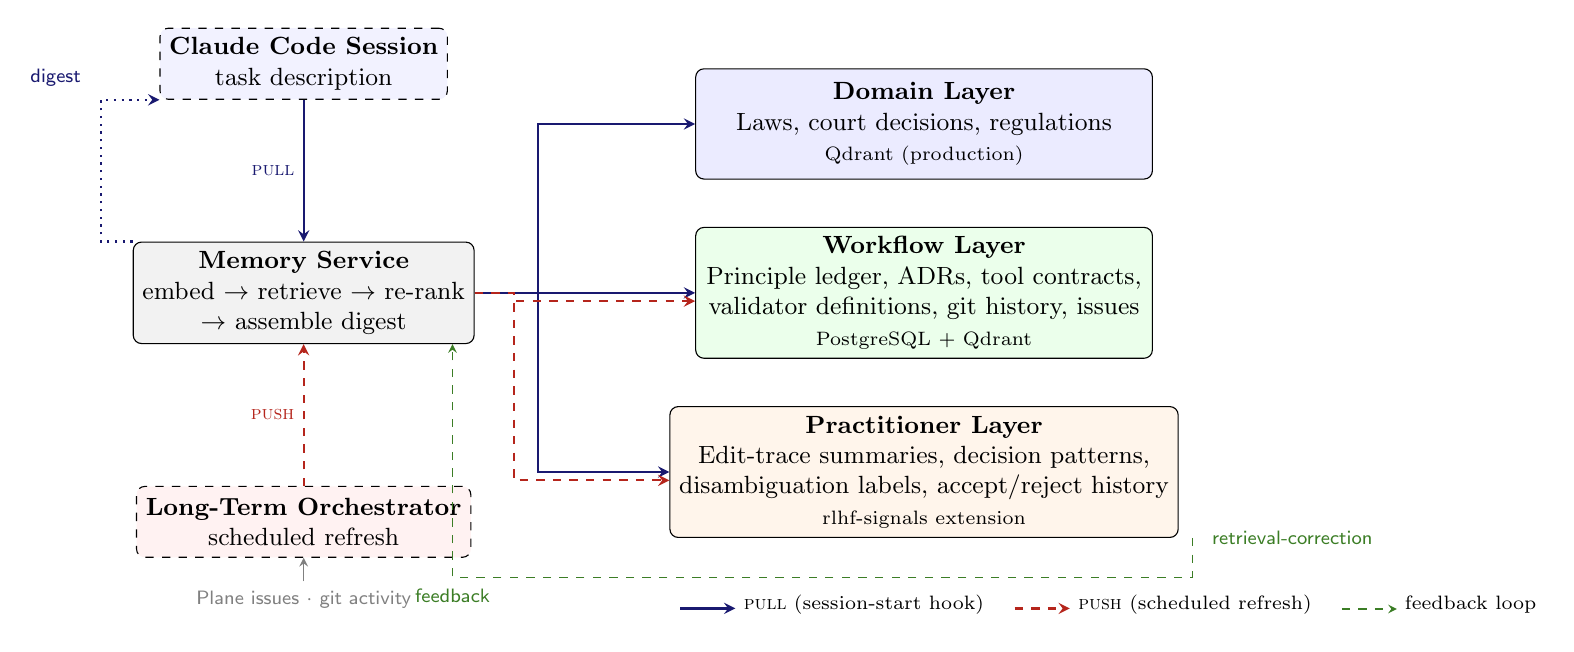
\begin{tikzpicture}[
    >=stealth,
    node distance=1.2cm and 2.0cm,
    layer/.style={draw, rounded corners=3pt, minimum width=5.8cm,
                  minimum height=1.4cm, align=center, font=\small},
    service/.style={draw, rounded corners=3pt, minimum width=3.8cm,
                    minimum height=1.0cm, align=center, font=\small},
    agent/.style={draw, dashed, rounded corners=3pt, minimum width=3.0cm,
                  minimum height=0.9cm, align=center, font=\small},
    pullpath/.style={->, thick, color=MidnightBlue},
    pushpath/.style={->, thick, color=BrickRed, dashed},
    labelbox/.style={font=\scriptsize\sffamily, fill=white, inner sep=1pt},
  ]

  % === Layers (right side) ===
  \node[layer, fill=blue!8] (domain)
    {\textbf{Domain Layer}\\Laws, court decisions, regulations\\{\scriptsize Qdrant (production)}};

  \node[layer, fill=green!8, below=0.6cm of domain] (workflow)
    {\textbf{Workflow Layer}\\Principle ledger, ADRs, tool contracts,\\
     validator definitions, git history, issues\\
     {\scriptsize PostgreSQL + Qdrant}};

  \node[layer, fill=orange!8, below=0.6cm of workflow] (practitioner)
    {\textbf{Practitioner Layer}\\Edit-trace summaries, decision patterns,\\
     disambiguation labels, accept/reject history\\
     {\scriptsize rlhf-signals extension}};

  % === Memory Service (center-left) ===
  \node[service, fill=gray!10, left=2.8cm of workflow] (memservice)
    {\textbf{Memory Service}\\embed $\rightarrow$ retrieve $\rightarrow$ re-rank\\$\rightarrow$ assemble digest};

  % === Claude Code session (top-left) ===
  \node[agent, fill=blue!5, above=1.8cm of memservice] (session)
    {\textbf{Claude Code Session}\\task description};

  % === Long-term orchestrator (bottom-left) ===
  \node[agent, fill=red!5, below=1.8cm of memservice] (orchestrator)
    {\textbf{Long-Term Orchestrator}\\scheduled refresh};

  % === Pull path (blue, solid) ===
  \draw[pullpath] (session.south) -- node[labelbox, left, xshift=-2pt]
    {\color{MidnightBlue}\textsc{pull}} (memservice.north);

  \draw[pullpath] (memservice.east) -- ++(0.8,0) |- (domain.west);
  \draw[pullpath] (memservice.east) -- (workflow.west);
  \draw[pullpath] (memservice.east) -- ++(0.8,0) |- (practitioner.west);

  % Return digest (pull)
  \draw[pullpath, dotted] (memservice.north west) -- ++(-0.4,0)
    |- node[labelbox, left, xshift=-6pt, yshift=8pt]
    {\color{MidnightBlue}digest} (session.south west);

  % === Push path (red, dashed) ===
  \draw[pushpath] (orchestrator.north) -- node[labelbox, left, xshift=-2pt]
    {\color{BrickRed}\textsc{push}} (memservice.south);

  \draw[pushpath] (memservice.east) -- ++(0.5,0) |- ([yshift=-3pt]workflow.west);
  \draw[pushpath] (memservice.east) -- ++(0.5,0) |- ([yshift=-3pt]practitioner.west);

  % === Issue tracker feed into orchestrator ===
  \node[font=\scriptsize\sffamily, below=0.3cm of orchestrator, text=gray]
    (tracker) {Plane issues $\cdot$ git activity};
  \draw[->, thin, gray] (tracker.north) -- (orchestrator.south);

  % === Retrieval-correction feedback loop ===
  \node[font=\scriptsize\sffamily, right=0.3cm of practitioner.south east,
        text=OliveGreen, anchor=west] (rcloop) {retrieval-correction};
  \draw[->, thin, OliveGreen, dashed]
    ([xshift=5pt]practitioner.south east) -- ++(0,-0.5)
    -| node[labelbox, below, yshift=-3pt] {\color{OliveGreen}feedback}
    ([xshift=-8pt]memservice.south east);

  % === Legend ===
  \node[anchor=north west, font=\scriptsize] at ([yshift=-0.6cm]practitioner.south west)
  {
    \tikz\draw[pullpath] (0,0) -- (0.7,0); \textsc{pull} (session-start hook) \quad
    \tikz\draw[pushpath] (0,0) -- (0.7,0); \textsc{push} (scheduled refresh) \quad
    \tikz\draw[->, thin, OliveGreen, dashed] (0,0) -- (0.7,0); feedback loop
  };

\end{tikzpicture}
\caption{Three-layer workflow memory architecture with dual-mode retrieval.
  \textsc{Pull} mode (solid blue) fires at session start: the task description is embedded
  and used to query all three Qdrant collections in parallel; results are re-ranked and
  assembled into a compact digest.
  \textsc{Push} mode (dashed red) runs on a schedule proportional to task activity,
  refreshing workflow and practitioner layer entries so that pull queries return current context.
  The retrieval-correction feedback loop (green) detects memory entries that \emph{should}
  have been retrieved but were not, feeding back into retrieval tuning and the RLHF
  pipeline as a process-level oversight signal.}
\label{fig:architecture}
\end{figure}


% --------------------------------------------------
\subsection{Domain Layer}
\label{sec:domain-layer}
% --------------------------------------------------

The domain layer contains the project's operational data: laws, court decisions, regulations, and other legal corpus material.
In the deployed system, this layer is already in production as multiple Qdrant vector collections served through MCP tools (semantic search, legislation retrieval, court decision lookup).

The architectural change is at the interface level.
Domain queries are routed through the memory service rather than directly to individual MCP tools.
This indirection provides three capabilities that direct tool calls lack: (1)~unified logging of all retrieval events, enabling retrieval-miss detection (Section~\ref{sec:retrieval-correction}); (2)~miss-rate measurement per collection, informing re-indexing priorities; and (3)~a uniform response format across all three layers, simplifying the digest assembly step.

The domain layer uses pure semantic retrieval: the query embedding is matched against document-chunk embeddings via cosine similarity, with optional metadata filtering (jurisdiction, date range, document type).

% --------------------------------------------------
\subsection{Workflow Layer}
\label{sec:workflow-layer}
% --------------------------------------------------

The workflow layer contains the project's decision context---the provenance that is absent from both code text and domain data.
Six sources populate this layer, listed in priority order:

\begin{enumerate}[leftmargin=*, nosep]
  \item \textbf{Principle ledger.} The highest-priority source. Each entry is a principle that the model violated and was corrected on---the hardest signal in the system. Entries are compact (typically one sentence plus metadata), referenced by validators (so retrievals are dense), and anchored to the constitutional framework described in the companion paper~\citep[\S5]{ovcharov2026recursive}. Schema: \texttt{id}, principle statement, severity (critical/warning/info), validator references, related ADR IDs, edit-trace links, embedding vector.

  \item \textbf{Validator definitions.} Source code of validation functions, parsed and embedded with docstrings, type signatures, and test examples. Validators encode the operational expression of constitutional principles; retrieving the validator alongside the principle provides the agent with both the ``what'' and the ``how.''

  \item \textbf{MCP tool contracts.} For each of the 70+ tools: name, description, parameter schema, example inputs and outputs. Embedded as structured text. Tool contracts evolve frequently in early development; the embedding pipeline re-indexes on each build.

  \item \textbf{ADR-style decision records.} One Markdown file per significant architectural decision, following Nygard's format~\citep{nygard2011adr}: context, decision, alternatives considered, consequences, related constitutional principles. Manually authored in Phase~1; automatic generation from PR descriptions is planned for Phase~2.

  \item \textbf{Git history with semantic enrichment.} For each merged PR: title, description, semantic class (from the companion paper's taxonomy), affected components, related ADR IDs. Provides temporal context for when and why code changed.

  \item \textbf{Issue tracker state.} Plane\footnote{\url{https://plane.so}} issues with state transitions, assignees, and linked PRs. Embedded with structured metadata to enable queries like ``what decisions were made on the billing migration?''
\end{enumerate}

The workflow layer uses hybrid retrieval: semantic similarity against embedded text, combined with structured filters on component, layer, severity, and temporal range.

% --------------------------------------------------
\subsection{Practitioner Layer}
\label{sec:practitioner-layer}
% --------------------------------------------------

The practitioner layer contains the practitioner's decision patterns, extracted from the same edit-trace pipeline described in the companion paper~\citep[\S3]{ovcharov2026recursive}.
This layer is the cross-reference point: the infrastructure that enables one practitioner to ship 1{,}547~PRs in 105 days \emph{generates} the preference signal the RLHF paper analyzes.

The layer never embeds raw content.
Following the privacy boundary established in the companion paper~\citep[\S6]{ovcharov2026recursive}, only structured edit summaries are indexed: edit class, semantic category, affected component, outcome (accepted/rejected/modified), and a one-sentence rationale generated by a nightly summarization job.
This preserves the separation between the practitioner's operational data (which may contain client-specific information) and the memory substrate (which contains only structured abstractions).

Retrieval is hybrid: semantic similarity combined with temporal and outcome-conditioned filtering.
A query about authentication patterns retrieves edit summaries where the practitioner corrected authentication-related code, ordered by recency and weighted by outcome confidence.

\paragraph{Phase~0: Prompt-Commit Bridge.}
Before the full practitioner layer, a minimal data collector is deployed: a \texttt{UserPromptSubmit} hook in Claude Code that creates an orphan commit in a bare git repository for every prompt.
Each record contains the prompt text, timestamp, session ID, repository, branch, and permission mode.
Over 4--6 weeks of passive collection, this yields a natural-text corpus for disambiguation labels, topic-frequency distributions, and cross-project switching patterns---the raw material for the practitioner layer's embedding pipeline.
Performance overhead is 15ms per capture, imperceptible within Claude Code's 5-second hook timeout.


% ============================================================
\section{Dual-Mode Retrieval}
\label{sec:dual-mode}
% ============================================================

The dual-mode retrieval architecture is the central contribution: pull-based retrieval for active sessions, push-based refresh for dormant tasks, operating as complementary mechanisms rather than alternatives.
Figure~\ref{fig:dual-mode} illustrates the interaction between both modes across a six-week horizon.

% Dual-mode timing diagram: pull and push interaction over a 6-week task
\begin{figure}[t]
\centering
\resizebox{\textwidth}{!}{%
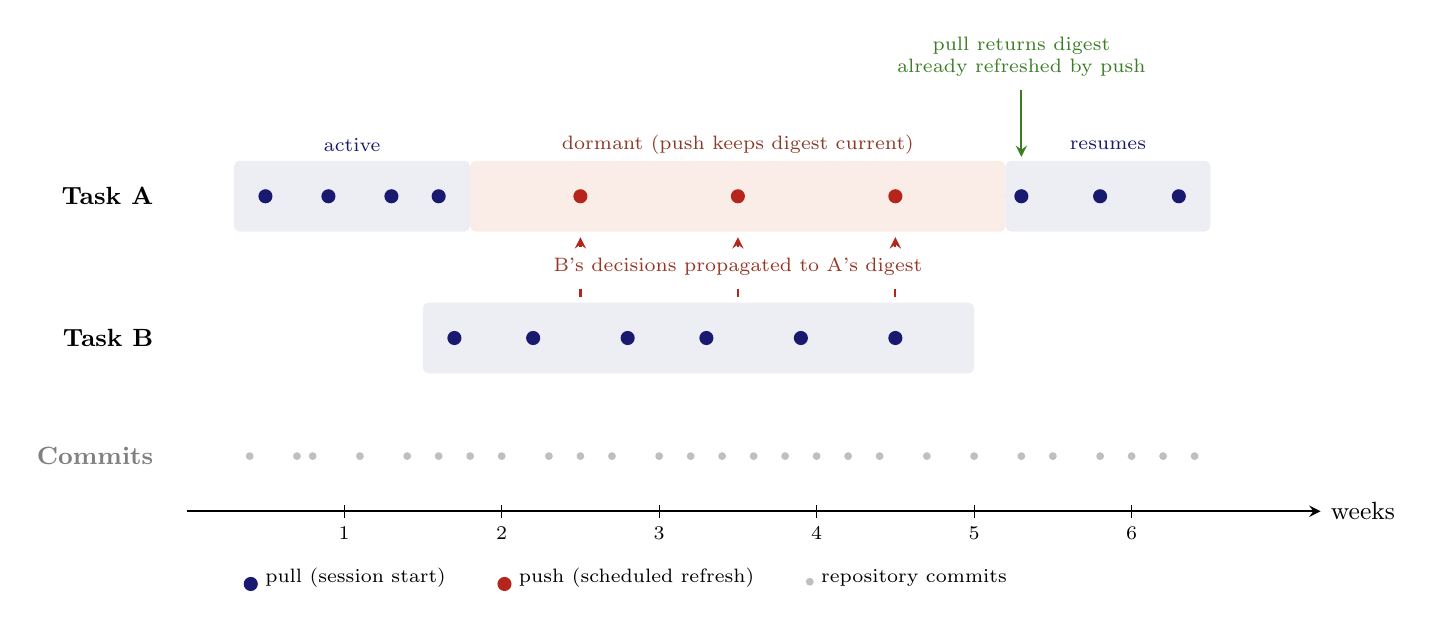
\begin{tikzpicture}[
    >=stealth,
    xscale=2.0,
    yscale=1.0,
    event/.style={circle, fill=#1, inner sep=1.8pt},
    pullev/.style={event=MidnightBlue},
    pushev/.style={event=BrickRed},
    commitdot/.style={event=gray!50, inner sep=1pt},
  ]

  % === Time axis ===
  \draw[->, thick] (0,-1.0) -- (7.2,-1.0) node[right, font=\small] {weeks};
  \foreach \w in {1,...,6} {
    \draw (\w, -0.92) -- (\w, -1.08) node[below, font=\scriptsize] {\w};
  }

  % === Task A timeline ===
  \node[font=\small\bfseries, anchor=east] at (-0.15, 3.0) {Task A};
  \draw[thick, gray!30] (0.3, 3.0) -- (6.5, 3.0);

  % Active/dormant shading
  \fill[MidnightBlue!8, rounded corners=2pt] (0.3, 2.55) rectangle (1.8, 3.45);
  \fill[BrickRed!6, rounded corners=2pt] (1.8, 2.55) rectangle (5.2, 3.45);
  \fill[MidnightBlue!8, rounded corners=2pt] (5.2, 2.55) rectangle (6.5, 3.45);

  % Phase labels above
  \node[font=\scriptsize, text=MidnightBlue] at (1.05, 3.65) {active};
  \node[font=\scriptsize, text=BrickRed!70!black] at (3.5, 3.65) {dormant (push keeps digest current)};
  \node[font=\scriptsize, text=MidnightBlue] at (5.85, 3.65) {resumes};

  % Pull events (blue dots)
  \foreach \x in {0.5, 0.9, 1.3, 1.6} { \node[pullev] at (\x, 3.0) {}; }
  \foreach \x in {5.3, 5.8, 6.3} { \node[pullev] at (\x, 3.0) {}; }

  % Push events (red dots, during dormancy)
  \foreach \x in {2.5, 3.5, 4.5} { \node[pushev] at (\x, 3.0) {}; }

  % === Task B timeline ===
  \node[font=\small\bfseries, anchor=east] at (-0.15, 1.2) {Task B};
  \draw[thick, gray!30] (1.5, 1.2) -- (5.0, 1.2);

  \fill[MidnightBlue!8, rounded corners=2pt] (1.5, 0.75) rectangle (5.0, 1.65);

  % Pull events
  \foreach \x in {1.7, 2.2, 2.8, 3.3, 3.9, 4.5} { \node[pullev] at (\x, 1.2) {}; }

  % === Cross-task propagation arrows ===
  \draw[->, BrickRed, thick, dashed, shorten >=2pt, shorten <=2pt]
    (2.5, 1.65) -- (2.5, 2.55);
  \draw[->, BrickRed, thick, dashed, shorten >=2pt, shorten <=2pt]
    (3.5, 1.65) -- (3.5, 2.55);
  \draw[->, BrickRed, thick, dashed, shorten >=2pt, shorten <=2pt]
    (4.5, 1.65) -- (4.5, 2.55);

  % Propagation label (single, centered)
  \node[font=\scriptsize, text=BrickRed!80!black, align=center, fill=white, inner sep=1.5pt]
    at (3.5, 2.1) {B's decisions propagated to A's digest};

  % === Key moment callout ===
  \draw[->, thick, OliveGreen] (5.3, 4.35) -- (5.3, 3.5);
  \node[font=\scriptsize, text=OliveGreen, align=center, anchor=south]
    at (5.3, 4.4) {pull returns digest\\already refreshed by push};

  % === Commit activity (bottom) ===
  \node[font=\small\bfseries, anchor=east, text=gray] at (-0.15, -0.3) {Commits};
  \foreach \x in {0.4, 0.7, 0.8, 1.1, 1.4, 1.6, 1.8, 2.0, 2.3, 2.5, 2.7, 3.0,
                   3.2, 3.4, 3.6, 3.8, 4.0, 4.2, 4.4, 4.7, 5.0, 5.3, 5.5, 5.8,
                   6.0, 6.2, 6.4} {
    \node[commitdot] at (\x, -0.3) {};
  }

  % === Legend ===
  \node[anchor=north west, font=\scriptsize] at (0.3, -1.6) {%
    \tikz[baseline=-0.5ex]\node[pullev] {};~pull (session start) \qquad
    \tikz[baseline=-0.5ex]\node[pushev] {};~push (scheduled refresh) \qquad
    \tikz[baseline=-0.5ex]\node[commitdot] {};~repository commits%
  };

\end{tikzpicture}%
}% end resizebox
\caption{Dual-mode retrieval over a six-week horizon with two concurrent tasks.
  Task~A is active in weeks~1--2, then dormant while Task~B runs in weeks~2--5.
  During dormancy, push-mode refresh propagates decisions from Task~B into Task~A's
  memory digest at a frequency proportional to commit activity.
  When Task~A resumes in week~5, the pull query returns context that is already current ---
  no expensive re-derivation required.
  Without push mode, the week-5 pull would return a stale digest from week~2, missing
  three weeks of relevant architectural decisions.}
\label{fig:dual-mode}
\end{figure}


% --------------------------------------------------
\subsection{Pull Mode}
\label{sec:pull-mode}
% --------------------------------------------------

Pull mode fires at session start via a Claude Code session-start hook.
The process:

\begin{enumerate}[leftmargin=*, nosep]
  \item The practitioner provides a task description (or the system infers it from the active Plane issue).
  \item The task description is embedded using the same model used for memory indexing (text-embedding-3-small or a locally hosted alternative such as bge-large-en-v1.5).
  \item Three parallel Qdrant queries execute against the domain, workflow, and practitioner collections, each with collection-specific filters (jurisdiction constraints for domain, component/severity for workflow, recency weighting for practitioner).
  \item Results from all three collections are merged and re-ranked using a cross-encoder~\citep{nogueira2019passage} or LLM-as-reranker, producing a unified relevance ordering.
  \item A greedy fill algorithm assembles the top-ranked entries into a token-budgeted digest, with a diversity constraint that ensures representation from all three layers.
\end{enumerate}

Latency target: $< 500$ms wall time for the full pipeline (embed, query, re-rank, assemble).
This is a design target, not a measurement; empirical latency will be reported after deployment.

% --------------------------------------------------
\subsection{Push Mode}
\label{sec:push-mode}
% --------------------------------------------------

Push mode runs as a scheduled orchestrator---a separate Docker container with a Bedrock Claude Sonnet summarization pipeline.
The orchestrator watches Plane tasks tagged \texttt{LONG-TERM} and refreshes their memory entries proportional to task activity.

The refresh frequency is a function of three signals:

\begin{equation}
  f_{\text{refresh}}(\text{task}) = g\bigl(
    \text{commits-touching-task},\;
    \text{comments-on-issue},\;
    \text{time-since-last-pull}
  \bigr)
  \label{eq:refresh}
\end{equation}

\noindent where $g$ is a monotonically increasing function of all three arguments, clamped to a maximum of one refresh per 24 hours and a minimum of one per 7 days for any task tagged \texttt{LONG-TERM}.

Each refresh produces three outputs:
\begin{itemize}[leftmargin=*, nosep]
  \item An \textbf{executive summary} of changes relevant to the task since the last refresh, generated by Bedrock Claude Sonnet from the diff of relevant commits and issue comments.
  \item A \textbf{tool lineage delta}: new tools created, tools modified, tools deprecated since the last refresh, with parameter-schema diffs.
  \item \textbf{Open questions}: unresolved issues or decision points flagged by the summarizer that may require practitioner input on task resumption.
\end{itemize}

The executive summary and tool lineage delta are embedded and stored in the workflow layer's Qdrant collection.
On the next pull query for the refreshed task, these entries surface alongside the original memory entries, providing the session with current context.

% --------------------------------------------------
\subsection{Why Both Modes Are Necessary}
\label{sec:why-both}
% --------------------------------------------------

Pull-only retrieval fails when a task is dormant for weeks and then resumes.
During the dormant period, other tasks' decisions accumulate relevant context: schema changes that affect the dormant task's data model, new constitutional principles that constrain its implementation, validator updates that redefine correctness criteria.
None of this context is incorporated into the dormant task's memory entries, because no pull query fires during dormancy.
When the task resumes, the pull query retrieves entries from the last active period---stale by weeks.
Re-deriving the current state requires expensive exploratory file reads, manual context assembly, and risk of missing cross-task dependencies.

Push-only refresh, conversely, is wasteful for active tasks.
A task with multiple sessions per day does not need pre-computed digests; each session's pull query returns current results because the memory entries were recently indexed.
Push refresh for active tasks duplicates the work that pull already performs, consuming Bedrock API credits without improving retrieval quality.

Dual-mode retrieval allocates computational effort where it provides the most value: pull for fast loops (active sessions), push for slow loops (dormant tasks).
The push mode is what makes 6-week horizons tractable; without it, retrieval over multi-week dormancy periods returns stale or absent context.

% --------------------------------------------------
\subsection{Retrieval-Correction Edits}
\label{sec:retrieval-correction}
% --------------------------------------------------

Retrieval-correction edits operationalize a specific oversight gap: the model produced an output that the practitioner corrected because the model's available context was missing information the practitioner had.
Definition: an edit where the model's output would have been correct given access to context~$X$, but $X$ was not present in the session's memory digest.
This edit class extends the six-class taxonomy from the companion paper~\citep[\S4]{ovcharov2026recursive}, but is structurally distinct: the other six classes capture \emph{what} the practitioner changed; retrieval-correction captures \emph{why} the change was avoidable.
It is therefore a process-level oversight signal rather than a preference signal in the standard RLHF sense.

Detection proceeds via a post-session reconciliation job:

\begin{enumerate}[leftmargin=*, nosep]
  \item After the session closes, the reconciliation job collects all edits made by the practitioner.
  \item For each substantive edit (edit distance $> 0.3$ in the companion paper's normalized metric), the job embeds the edit context and queries the memory store for entries that are semantically similar to the edit but were \emph{not} retrieved in the session's digest.
  \item Candidate retrieval-correction pairs (edit, unretrieved-but-relevant memory entry) are flagged for practitioner review.
  \item Confirmed pairs are labeled as retrieval-correction edits and enter the alignment pipeline as oversight-derived preferences: the ``chosen'' response incorporates the missing context; the ``rejected'' response is the original model output that lacked it.
\end{enumerate}

This closes a feedback loop between the memory layer and the alignment pipeline that is structurally different from outcome-level RLHF.
Outcome-level supervision answers ``did this run succeed?'' once per session.
Retrieval-correction supervision answers ``was this specific output reachable from this specific context?'' per edit.
The signal density per unit of agent activity is therefore higher, and the signal is invariant to session length.
Two consequences follow.
First, as the memory layer matures, retrieval-correction edit rate becomes a measurable proxy for memory effectiveness---an internal evaluation metric that does not require waiting for downstream outcomes.
Second, retrieval-correction edits encode a failure mode (capability present, context absent) that is distinct from capability gaps (capability absent, context irrelevant).
Distinguishing these failure modes is a long-standing open problem in scalable oversight~\citep{bowman2022scalable}; the memory layer provides one concrete instantiation.


% ============================================================
\section{Implementation}
\label{sec:implementation}
% ============================================================

The memory service is implemented in TypeScript, consistent with the existing Express-based MCP backend~\citep{anthropic2024mcp} described in the companion paper~\citep[\S7]{ovcharov2026recursive}.
The technology stack reuses production infrastructure: Qdrant for vector storage, PostgreSQL for structured metadata (new \texttt{workflow\_memory\_*} tables), Redis for caching, and AWS Bedrock Claude Sonnet for summarization steps.

% --------------------------------------------------
\subsection{Memory Query Tool}
\label{sec:memory-query-tool}
% --------------------------------------------------

A single MCP tool, \texttt{workflow\_memory\_query}, serves as the primary retrieval interface.
Parameters:

\begin{itemize}[leftmargin=*, nosep]
  \item \texttt{task\_description} (string, required): natural-language description of the current task.
  \item \texttt{scope} (enum: \texttt{all} | \texttt{domain} | \texttt{workflow} | \texttt{practitioner}): which layers to query. Default: \texttt{all}.
  \item \texttt{token\_budget} (integer, default 8{,}000): maximum tokens in the assembled digest.
  \item \texttt{filters} (object, optional): structured filters (component, severity, date range).
\end{itemize}

The tool returns a structured prose digest with section headers per layer, relevance scores per entry, and source provenance links.
The digest format is designed for direct injection into the agent's context window without post-processing.

% --------------------------------------------------
\subsection{Long-Term Task Orchestrator}
\label{sec:orchestrator}
% --------------------------------------------------

The push-mode orchestrator runs as a separate Docker container with its own cron schedule.
It queries the Plane API for tasks tagged \texttt{LONG-TERM}, computes refresh priority per Equation~\ref{eq:refresh}, and dispatches summarization jobs to Bedrock.
Outputs (executive summaries, tool lineage deltas, open questions) are embedded and stored in the workflow layer's Qdrant collection with a \texttt{source: push-refresh} metadata tag.

Implementation proceeds in five phases over 11 weeks; details are available in the supplementary materials.\footnote{Phase schedule: \url{https://github.com/overthelex/SecondLayer/blob/main/docs/workflow-memory-phases.md}}


% ============================================================
\section{Evaluation Plan}
\label{sec:evaluation}
% ============================================================

% --------------------------------------------------
\subsection{Metrics}
\label{sec:metrics}
% --------------------------------------------------

Four metrics operationalize the architecture's success criteria, each paired with a baseline measurement method and a target.

\begin{table}[h]
\centering
\small
\begin{tabularx}{\textwidth}{@{}l X c c@{}}
\toprule
\textbf{Metric} & \textbf{Measurement method} & \textbf{Baseline} & \textbf{Target} \\
\midrule
Session file reads &
  Count Read tool calls per session across 304 sessions from companion dataset &
  23.1 (mean) & ${\leq}8$ \\
\addlinespace
Session bootstrap (input tokens) &
  Sum input tokens at first API call; $N{=}304$ sessions &
  30{,}115 (median) & ${\leq}10$K \\
\addlinespace
Context waste ratio &
  Files read but never edited / total files read; $N{=}180$ sessions with ${\geq}3$ reads &
  60\% (median) & ${\leq}20\%$ \\
\addlinespace
Principle retrieval accuracy &
  Held-out set of principle ledger entries; queries derived from edit-traces that originally triggered each principle &
  n/a & ${\geq}80\%$ \\
\addlinespace
Long-term task refresh latency &
  Time from relevant commit to updated digest entry &
  n/a (no automation) & ${\leq}24$h \\
\bottomrule
\end{tabularx}
\caption{Evaluation metrics with measured baselines and targets.
  Bootstrap baselines are measured from 304 Claude Code sessions in the companion paper's transcript dataset.}
\label{tab:metrics}
\end{table}

A fifth metric---the retrieval-correction edit rate over time---is qualitative in Phase~1.
As the practitioner layer matures, the rate of retrieval-correction edits (Section~\ref{sec:retrieval-correction}) should decrease.
The expected trajectory is a declining curve over the first 6--8 weeks of deployment, flattening as the memory layer covers the most frequently needed context.

% --------------------------------------------------
\subsection{Preliminary Results}
\label{sec:preliminary}
% --------------------------------------------------

Three baseline measurements are available at submission time, derived from the companion paper's transcript dataset and from the project's git history.

\paragraph{Bootstrap cost (Experiment~1, $N{=}304$ sessions).}
Parsing Claude Code API transcripts from the companion dataset, the median first-call input token count is 30{,}115 (mean 29{,}693; $\sigma{=}7{,}594$; P10/P90: 18{,}540/41{,}774).
Of these, ${\sim}17{,}600$ tokens (59\%) are cache-creation cost for \texttt{CLAUDE.md} and system context---loaded unconditionally on every session regardless of task.
Per-session file reads (Read tool calls) average 23.1 (median~14, P90: 61), but 72\% of sessions have zero Read calls in the bootstrap phase; most sessions open with shell commands (\texttt{git status}, \texttt{ls}) rather than file reads.
The memory layer's primary reduction target is therefore the automatic context cost ($T$), not the file-read count.

\paragraph{CLAUDE.md growth (Experiment~2, 25~commits over 85~days).}
The project's \texttt{CLAUDE.md} grew from 4{,}099 to 24{,}148 characters (152 to 474~lines) across 25 commits spanning January~17 to April~12, 2026.
A linear regression of character count on days elapsed yields a slope of 216.7~chars/day with $R^2 = 0.87$, confirming the approximately linear growth claimed in Section~\ref{sec:intro}.
Line count is noisier ($R^2 = 0.58$) due to periodic reformatting that changes density without changing content volume.

\paragraph{Context waste ratio (Experiment~3, $N{=}180$ sessions).}
Across sessions with at least three file reads in the bootstrap phase (first 50~turns), the median context waste ratio---files read but never subsequently edited in the session---is 60\% (mean 56.7\%; $\sigma{=}26.3\%$).
The distribution is right-skewed: 66\% of sessions waste more than half their bootstrap reads; only 15\% waste less than 30\%.
Source-code reads are wasted at 78\%, while memory files (\texttt{.claude/memory/}) are wasted at 66.5\%, suggesting that structured memory retrieval is more targeted than exploratory file reads.
Waste ratio correlates negatively with session length: short sessions (5--10 turns) waste 68.5\%; longer sessions ($>$50 turns) waste 51.1\%.

\paragraph{Phase~0 status.}
The prompt-commit bridge has been deployed since May~9, 2026 and has captured 23~prompts across 5~sessions and 4~repositories.
Meaningful distributional analysis (topic clustering, cross-project switching rates) requires 4--6 weeks of passive collection.

Full evaluation of the memory layer itself (retrieval accuracy, bootstrap reduction with memory enabled) will be reported after Phase~1.3 deployment.

% --------------------------------------------------
\subsection{Threats to Validity}
\label{sec:threats}
% --------------------------------------------------

\paragraph{Single project, single practitioner.}
The architecture is designed and evaluated in the context of one project (LEX AI) and one practitioner.
This is the same constraint as the companion RLHF paper~\citep[\S8]{ovcharov2026recursive}.
Mitigation: the architecture is project-agnostic---the three-layer decomposition and dual-mode retrieval impose no assumptions about the domain, the programming language, or the practitioner's expertise.
Generalization claims are deferred to Phase~2, which introduces a multi-practitioner cohort.

\paragraph{Confounding with codebase maturity.}
Bootstrap reduction could result from caching effects, improved \texttt{CLAUDE.md} curation, or the natural stabilization of a maturing codebase rather than from the memory layer itself.
Control: A/B evaluation by toggling the memory layer at session start.
Sessions with the memory layer enabled are compared against sessions without it on the same task distribution during the same time period.

\paragraph{Principle ledger quality.}
In Phase~1, the principle ledger is human-curated.
Retrieval accuracy is therefore bounded by curation quality, not retrieval quality.
If the registry is incomplete or contains imprecise principle statements, the retrieval system will faithfully return imprecise results.
This limitation is acknowledged and addressed in Phase~2 by introducing semi-automatic principle extraction from edit-traces.


% ============================================================
\section{Discussion}
\label{sec:discussion}
% ============================================================

\paragraph{Memory layer as RLHF substrate.}
The same infrastructure that enables one practitioner to ship 1{,}547~PRs in 105~days \emph{generates} the preference signal the companion paper analyzes.
Memory and preference data are two views of the same long-horizon work: a retrieval-correction edit is simultaneously a memory-layer failure (the system did not surface relevant context) and an alignment signal (the practitioner corrected the model's output, producing a preference pair).
This duality is not incidental---it is the architectural thesis.
The memory layer does not merely consume alignment data; it produces it.

\paragraph{Memory as scalable oversight surface.}
The memory layer is dual-purpose: it serves the agent during execution and generates oversight signal during reconciliation.
As agent autonomy grows---from short interactive sessions to multi-hour autonomous runs to multi-day autonomous projects of the kind documented in Anthropic's long-running scientific computing work~\citep{anthropic2026longrunning}---the ratio of practitioner-observable outcomes to agent-internal decisions falls.
Outcome-level supervision becomes a low-bandwidth channel through which any oversight signal must pass.

The memory layer changes this.
Every retrieval is an observable event with a known context window, a known retrieval result, and a subsequent edit trace.
Reconciliation between retrieved context and editing behavior generates oversight signal at the granularity of individual edits, not individual sessions.
The signal is not free---reconciliation requires practitioner confirmation of candidate retrieval-correction pairs---but the practitioner's marginal cost per signal is bounded by the time to confirm a flagged pair, not the time to evaluate an entire session.

This positions the memory layer as one concrete answer to the question posed in \emph{Recommendations for Technical AI Safety Research Directions}~\citep{anthropic2025recommended}: how to design oversight mechanisms whose signal scales with the systems they oversee.
The architecture does not solve scalable oversight in general.
It demonstrates that for one operational regime---long-horizon agentic coding by a small number of practitioners---the memory infrastructure that makes the regime tractable also produces the signal needed to oversee it.

\paragraph{Generalization to teams.}
The architecture as described serves a single practitioner.
Multi-practitioner deployment introduces three challenges not addressed here: (1)~multi-writer principle ledger with conflict resolution on principle updates; (2)~per-practitioner views of the practitioner layer, since different practitioners have different correction patterns; and (3)~access control on memory entries that may contain project-specific context.
These are Phase~2 concerns.
The three-layer decomposition is designed to accommodate them---the domain layer is already shared, the workflow layer supports scoped views via metadata filtering, and the practitioner layer is inherently per-practitioner.

\paragraph{What this is not.}
The workflow memory architecture is not a replacement for long-context models; it is a retrieval substrate that reduces the context a long-context model must process.
It is not a knowledge graph: there is no formal ontology, no RDF triples, no SPARQL endpoint.
It is not an enterprise knowledge management system: it has no document lifecycle, no approval workflows, no compliance metadata.
It is a retrieval substrate optimized for one operational regime---long-horizon agentic composition by a small number of practitioners---and its design decisions reflect that specificity.


% ============================================================
\section{Limitations}
\label{sec:limitations}
% ============================================================

\begin{itemize}[leftmargin=*, nosep]
  \item \textbf{Single project, single practitioner.} All design and evaluation is within one legal-technology project built by one practitioner. Generalization to other domains, other languages, or multi-developer teams is not demonstrated.

  \item \textbf{Manual ADR curation.} In Phase~1, architecture decision records are manually authored. The curation burden is non-trivial at 14.7~PRs/day; ADR coverage is expected to be incomplete during the evaluation period.

  \item \textbf{Batch re-indexing.} Memory entries are re-indexed nightly, not in real time. Changes made during a session are not reflected in the memory layer until the next indexing run. This creates a window where pull queries may return slightly stale results for very recent changes.

  \item \textbf{No multi-practitioner support.} The architecture does not address multi-writer conflicts in the principle ledger, per-practitioner memory views, or cross-practitioner preference aggregation.

  \item \textbf{Retrieval-correction detection is approximate.} The post-session reconciliation job uses semantic similarity to identify candidate retrieval-correction pairs. False positives (flagged pairs where the missing context would not have changed the model's output) are filtered by practitioner review, but the detection precision is not yet measured.

  \item \textbf{Push-mode cost.} Each push refresh consumes Bedrock API credits for summarization. At scale, the cost of maintaining current digests for many dormant tasks may become significant. The current design mitigates this with frequency clamping (maximum one refresh per 24 hours per task), but cost-optimal refresh scheduling is not formalized.

  \item \textbf{Oversight-signal density is not yet quantified.} The claim that retrieval-correction edits constitute a denser oversight signal than outcome-level supervision is structurally argued but not measured. Quantifying signal density (retrieval-correction edits per practitioner-minute vs.\ outcome labels per practitioner-minute) requires the full deployment to run for several weeks; this measurement is part of the evaluation plan.
\end{itemize}


% ============================================================
\section{Conclusion}
\label{sec:conclusion}
% ============================================================

This paper presented a workflow memory architecture for long-horizon agentic composition, addressing the session bootstrap problem that bottlenecks multi-week LLM-assisted software engineering.
Three contributions were made.
First, a three-layer memory decomposition---domain, workflow, and practitioner---where each layer has distinct content, retrieval semantics, and storage substrate, and the retrieval unit is the architectural decision rather than the code chunk or dialogue turn.
Second, dual-mode retrieval as a first-class primitive: pull mode for active sessions, push mode for dormant tasks, with push-mode refresh keeping multi-week horizons tractable by maintaining current memory entries without requiring active sessions.
Third, retrieval-correction edits as a process-level oversight signal that scales with agent autonomy, closing the feedback loop between the memory layer and the alignment pipeline described in the companion paper~\citep{ovcharov2026recursive}.

The architecture is deployed incrementally on a production legal-technology platform.
Phase~0 (prompt-commit bridge) is live; Phases~1.0--1.5 are in implementation.
Baseline measurements from 304 sessions confirm a median bootstrap cost of 30{,}115 input tokens and a context waste ratio of 60\%; the memory layer targets ${\leq}10$K tokens and ${\leq}20\%$ waste, with ${\geq}80\%$ retrieval accuracy on principle ledger entries.

The source code and implementation notes are available at \url{https://github.com/overthelex/SecondLayer}.


% ============================================================
%  References
% ============================================================
\bibliographystyle{plainnat}
\bibliography{references}

\end{document}
